\documentclass{article}
\usepackage{graphicx}
\usepackage[utf8]{inputenc}

\graphicspath{ {./images/} }

\title{Creazione di un demodulatore di segnale FM simulato in software}
\author{Lena Giovanni Leonardo}
\date{15 Febbraio 2022}

\begin{document}

\maketitle

\section{Introduction}

\subsection{Segnale FM}
La modulazione FM è una modulazione che consente di codificare un segnale detto modulante all'interno di un altro segnale di frequenza
più alta detto portante. L'informazione del segnale modulante è contenuto nella variazione di frequenza. Il segnale modulato
ha quindi un'ampiezza costante ma una frequenza che varia. La modulazione FM è usata spesso quando si vuole trasmettere un segnale
a bassa frequenza attraverso onde radio.

\subsection{Tecnica DSP}
DSP o Digital Signal Processing consiste nell'elaborazione di un segnale utilizzando tecniche software, spesso emulando un circuito.
La comodità di questa tecnica è che un computer può emulare qualsiasi circuito ed è quindi molto più flessibile.

\section{I segnali di partenza}
La prima simulazione è realizzata in Python con il software Jupyter Lab che permette di eseguire 
parti di codice e visualizzarne immediatamente i risultati tramite grafici e tabelle. Il codice 
scritto in Python sarà poi importato all'interno di LabVIEW.
\\
Prima di demodulare un segnale FM è necessario avere un segnale FM, il quale si crea a partire da un segnale 
modulante ed uno portante. In questo esempio i due segnali sono entrambi sinusoidali, quello modulante ha una 
frequenza $f_m = 1 kHz$ mentre quello portante ha una frequenza di $f_m = 10 kHz$.
\\
Avvalendosi degli strumenti di visualizzazione di Jupyter Lab, è possibile visualizzare il grafico dei due segnali:
\\
\begin{center}
    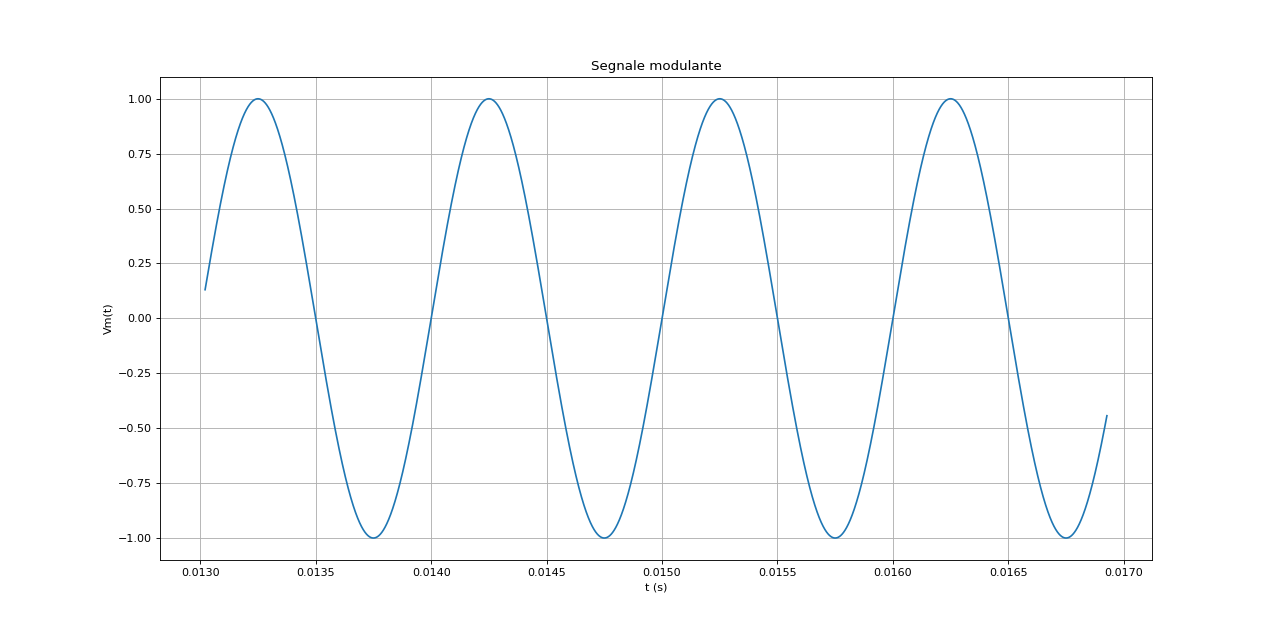
\includegraphics[width=\textwidth]{modulante.png}
\end{center}
Il segnale modulante, $f = 1 kHz$

\begin{center}
    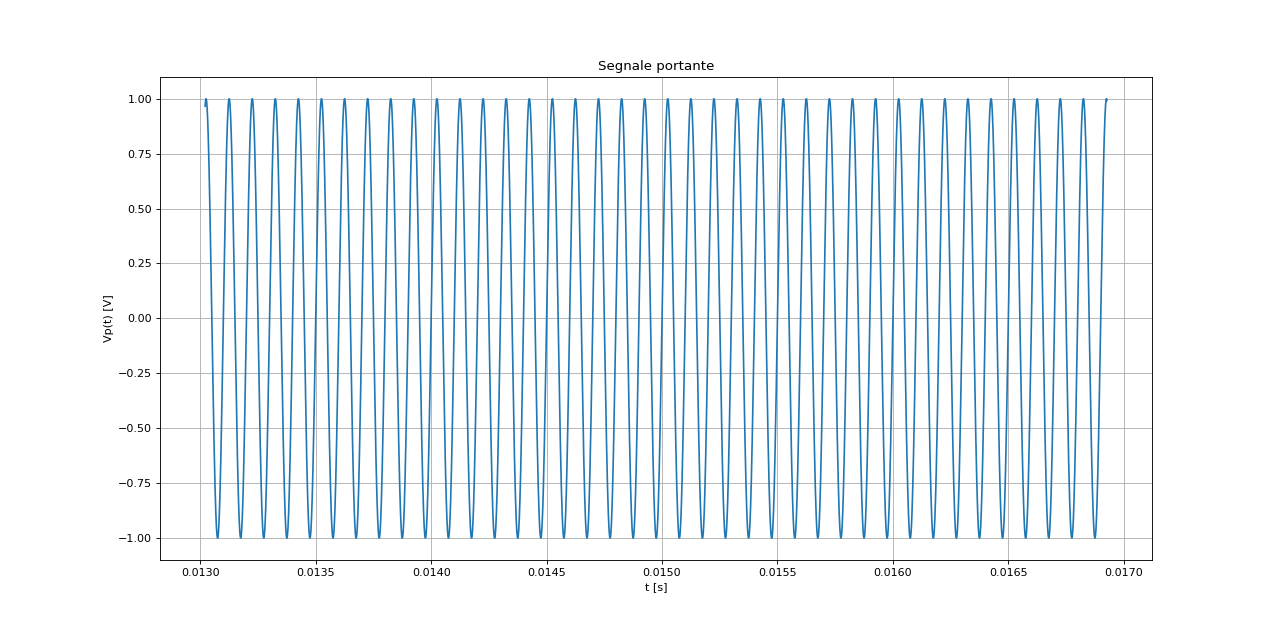
\includegraphics[width=\textwidth]{portante.png}
\end{center}
Il segnale portante, $f = 10 kHz$

\newpage
Che uniti vengono modulati nel seguente segnale FM.

\begin{center}
    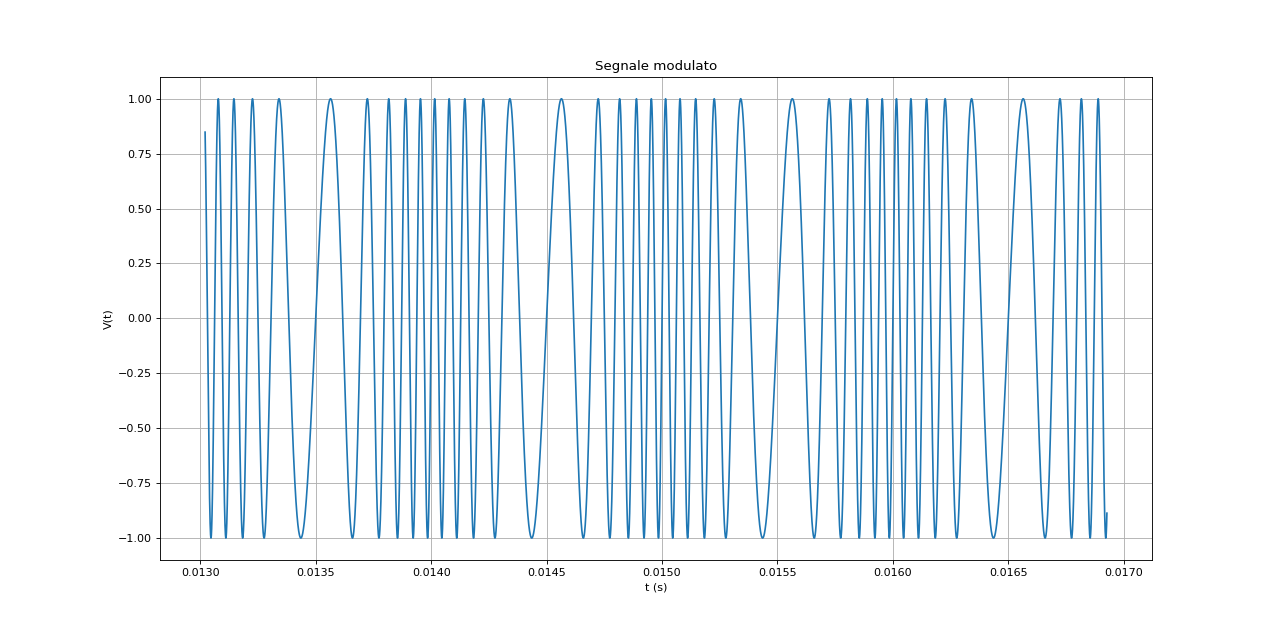
\includegraphics[width=\textwidth]{modulato.png}
\end{center}


\section{Implementazione in DSP}
\subsection{Filtro passa basso}
Per demodulare un segnale FM è necessario applicare un filtro passa-basso. In hardware si potrebbe implementare
con un circuito R-C, mentre in software è sufficiente scrivere un algoritmo che discretizza il circuito.\\
L'implementazione più semplice richiede un ciclo for e si può scrivere in Python con la seguente funzione:

\begin{verbatim}
def low_pass_filter(signal: List[float], tau: float) -> List[float]:
    output = np.zeros_like(signal)

    output[0] = tau * signal[0]
    for i in range(1, len(modulated)):
        output[i] = output[i - 1] + tau * (signal[i] - output[i - 1])

    return output
\end{verbatim}

La funzione prende in input un segnale e una tau, e ritorna il segnale filtrato.

Per testare il corretto funzionamento del filtro passa basso, genero un segnale sinosoidale
con frequenza crescente, da $0 Hz$ a $1900 Hz$ e applico il filtro passa basso.

\begin{center}
    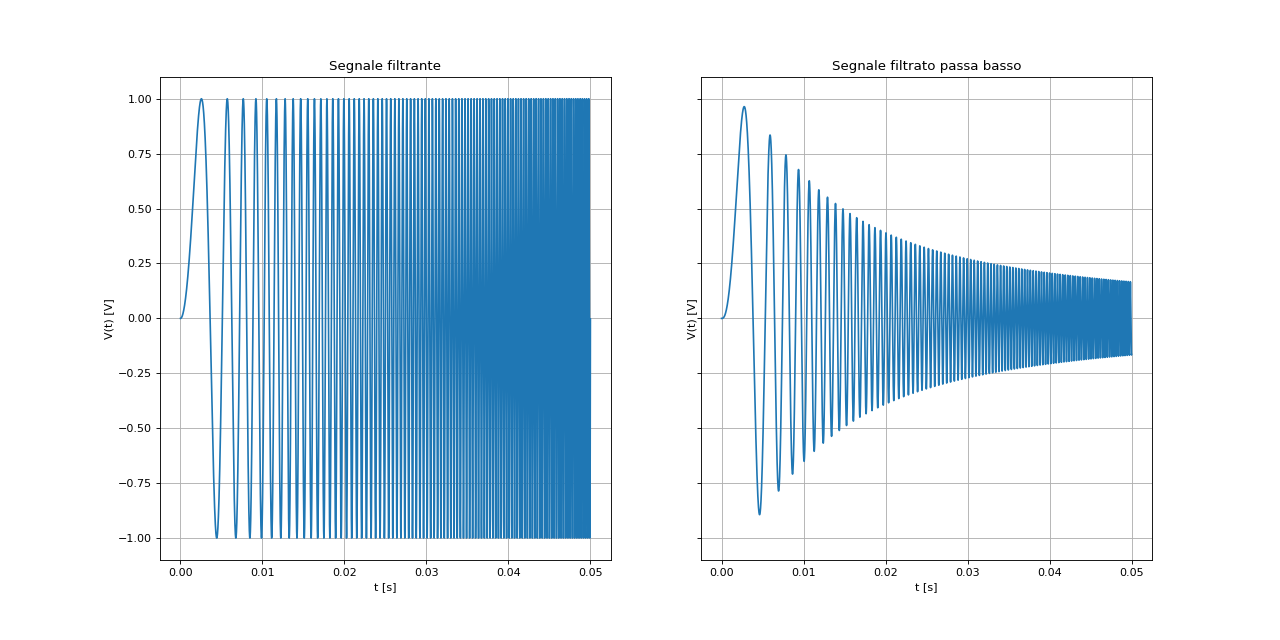
\includegraphics[width=\textwidth]{filtrato-test.png}
\end{center}

Come evidente dal grafico a destra, il segnale viene filtrato correttamente e le frequenze superiori
alla frequenza di taglio vengono attenuate, come ogni filtro passa basso di primo ordine.

\subsection{Diodo}
Per simulare un diodo è sufficiente applicare la funzione di valore assoluto al segnale. In Python
è sufficiente applicare al segnale la funzione abs.

\begin{verbatim}
def diode(signal: List[float]) -> List[float]:
    return [abs(s) for s in signal]
\end{verbatim}

Anche in questo caso, per verificarne il corretto funzionamento è sufficiente inserire un segnale
sinusoidale e verificarne l'output.

\begin{center}
    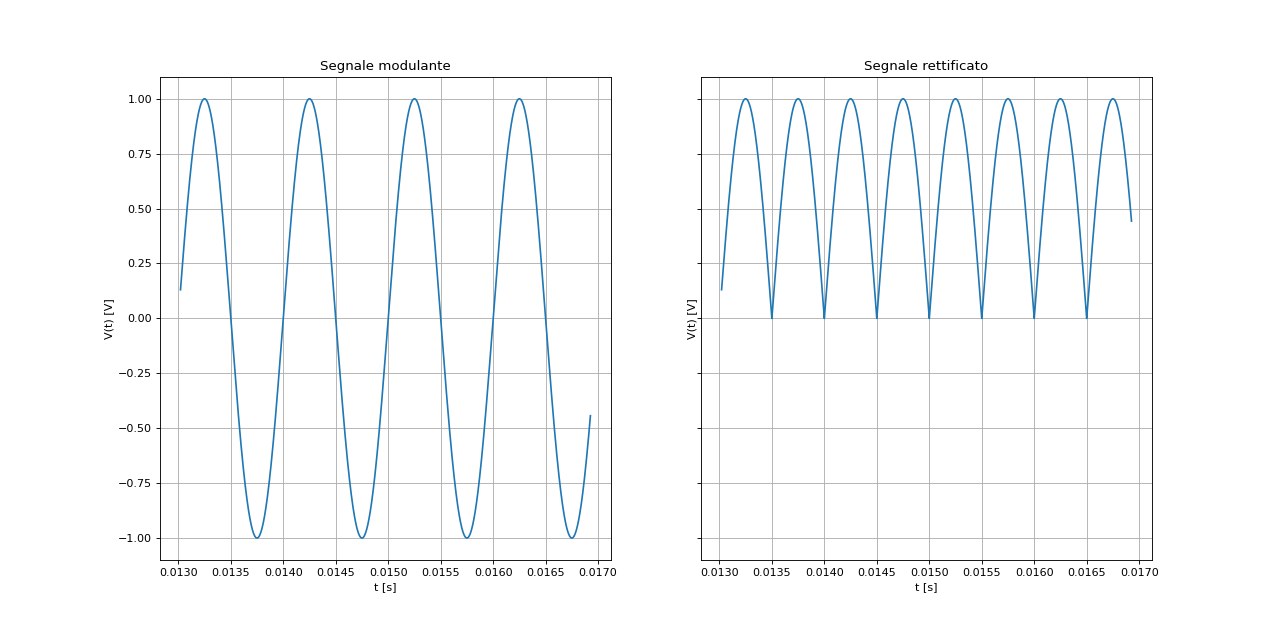
\includegraphics[width=\textwidth]{diode.png}
\end{center}

\section{Demodulazione in Python}

\subsection{Filtro passa basso}
Per poter tornare al segnale modulante di partenza, il primo passo è quello di applicare un filtro passa-basso.
Nel caso concreto, la frequenza di taglio del filtro è pari al 70\% della frequenza della portante, che in 
questo caso è pari a $7 kHz$.
\\
Applicando la funzione creata in precedenza, si ottiene in output un segnale pseudo-AM.

\begin{center}
    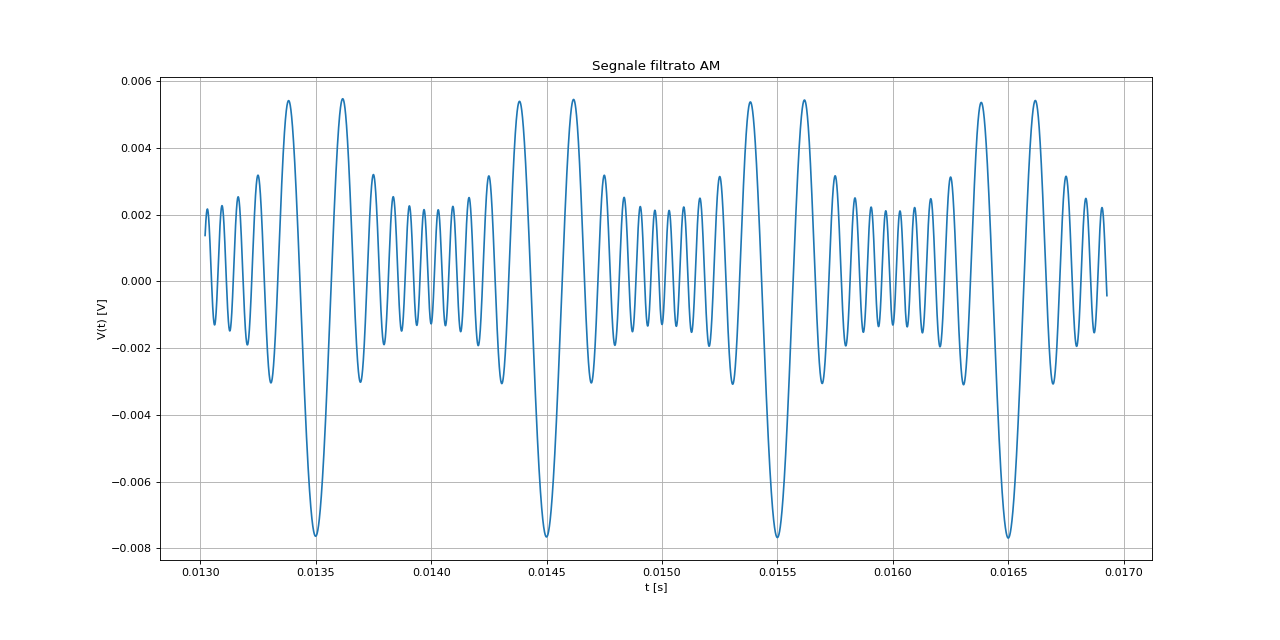
\includegraphics[width=\textwidth]{filtrato.png}
\end{center}

\subsection{Semionda positiva}
Il secondo passaggio consiste nell'ottenere solamente la semionda positiva del segnale AM. Per far ciò è sufficiente
applicare la funzione diode definita precedentemente.

\begin{center}
    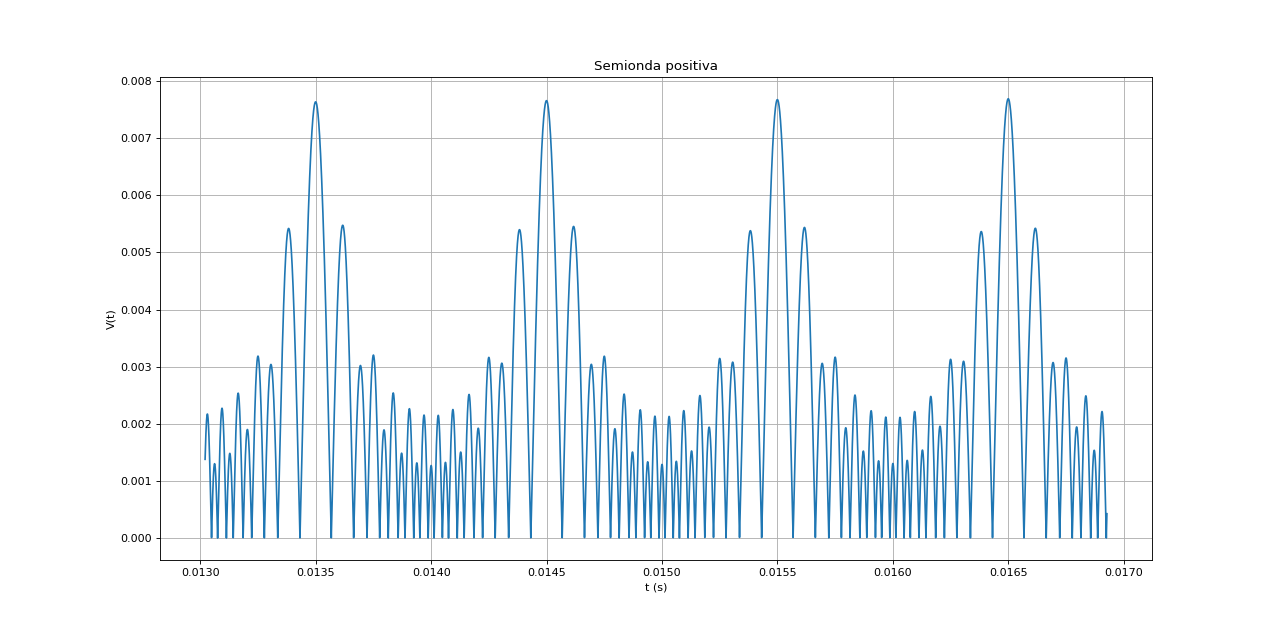
\includegraphics[width=\textwidth]{positivo.png}
\end{center}

\subsection{Rilevatore di inviluppo}
Per ottenere indietro il segnale modulante, si applica un cosiddetto rilevatore di inviluppo, che non è altro che un filtro
passa basso che segue i "picchi" del segnale, togliendo tutta la cosiddetta seghettatura.
\\
La frequenza di taglio del filtro passa basso in questo caso è pari a tre volte la frequenza modulante, ovvero $3 kHz$.
Avendo già la funzione pronta per il passa basso, è sufficiente chiamarla passando come parametri il segnale della semionda
positiva e la tau relativa a $3 kHz$.
\\
Sottraendo poi un segnale DC per centrare lo zero del segnale ed avere una parte positiva ed una negativa, si ottiene finalmente
un'onda che assomiglia molto alla sinusoide di partenza.

\begin{center}
    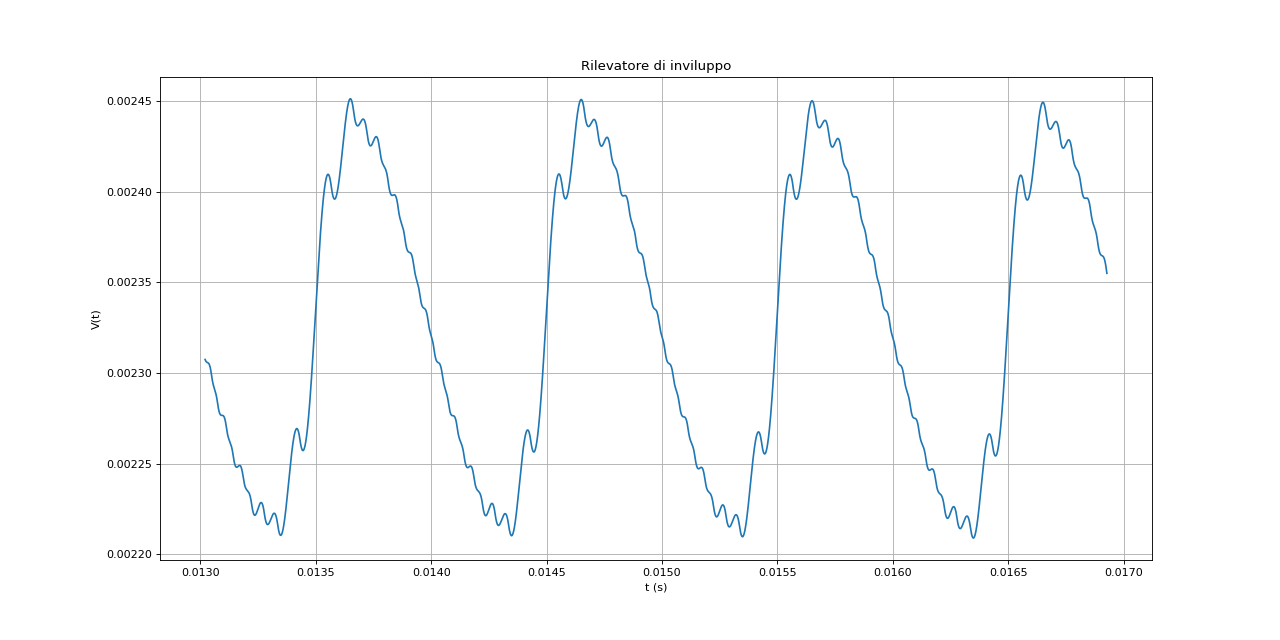
\includegraphics[width=\textwidth]{inviluppo.png}
\end{center}
Il segnale demodulato.

\begin{center}
    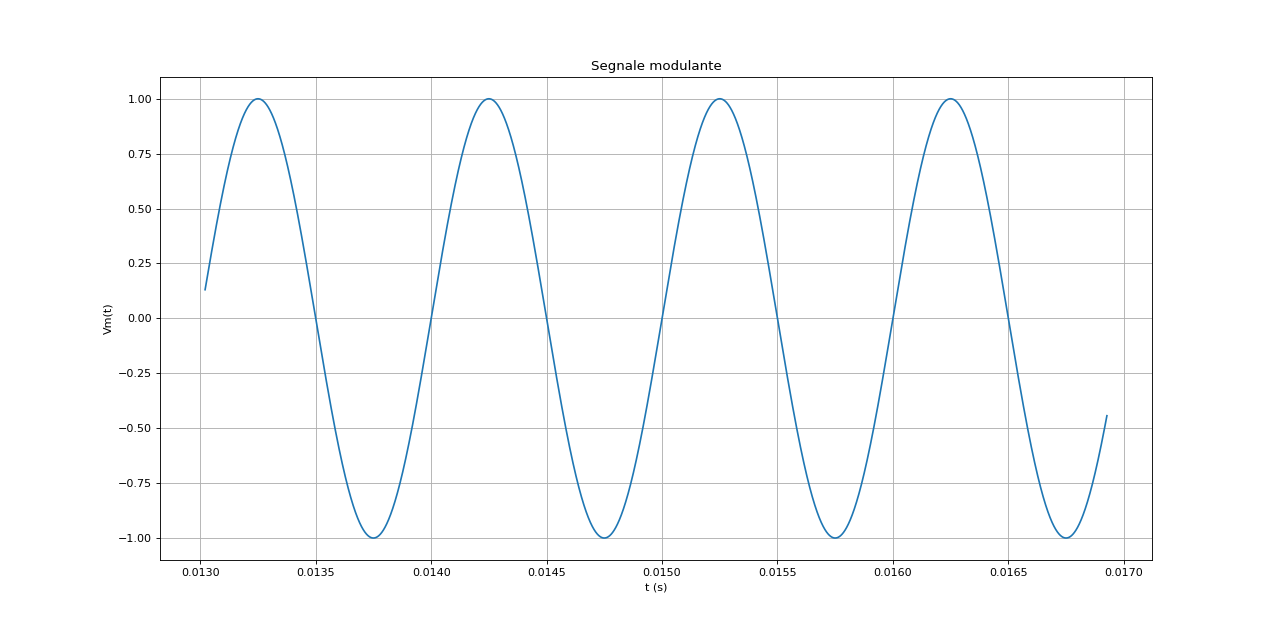
\includegraphics[width=\textwidth]{modulante.png}
\end{center}
Il segnale modulante di partenza.

\vspace{2cm}
Come si può facilmente notare confrontando i due segnali, il primo è sfasato di 180 gradi rispetto al secondo.
Si tratta probabilmente del risultato dei due filtri passa-basso di primo ordine, che oltre ad attenuare il segnale
applicano anche uno sfasamento.

\section{Implementazione in LabVIEW}
LabVIEW permette di eseguire codice Python, per cui è possibile importare il codice già scritto ed eseguirlo per ottenere
il segnale demodulato.

\end{document}
